% Detour Steer - short summary (English). Build: pdflatex (twice), inside algorithm_sim/docs
\documentclass[11pt,a4paper]{article}
\usepackage[T1]{fontenc}
\usepackage[top=1.6cm,bottom=1.6cm,left=2cm,right=2cm]{geometry}
\usepackage{mathpazo}
\usepackage{amsmath,amssymb}
\usepackage{booktabs}
\usepackage[linesnumbered,lined]{algorithm2e}
\usepackage{graphicx}
\usepackage{url}
\usepackage[hidelinks]{hyperref}
\RestyleAlgo{boxed}
\SetAlgoNlRelativeSize{-1}
\newcommand{\algcommentfont}[1]{\footnotesize\textnormal{#1}}
\SetCommentSty{algcommentfont}
\SetKwComment{tcp}{/\kern-0.12em/\ }{}
\SetKwProg{Pro}{Procedure :}{}{end}
\SetKw{KwNone}{None}
\SetKw{KwOr}{or}
\SetFuncSty{textit}
\SetKwFunction{FPlan}{PlanLeg}
\setlength{\parindent}{0pt}
\setlength{\parskip}{3pt}
\usepackage{titlesec}
\titlespacing*{\section}{0pt}{2.2ex}{0.8ex}
\pagestyle{empty}

\begin{document}
\begin{flushright}{\small\bfseries Phuthiphong Wongchantib 660610840}\end{flushright}
\vspace{-3mm}
\begin{center}
{\Large\bfseries Detour Steer --- Summary}\\[1mm]
Decision algorithm for a robot that steers one way only: drive on, steer less, come back
\end{center}

\section*{1. Problem}
The robot \texttt{mor\_luam} has \textbf{one motor}. Turning it one way \emph{steers} the wheel
(counter-clockwise only). Turning it the other way \emph{drives} forward. So the robot must
\textbf{stop to steer} and can never steer while it drives.
The old method steers straight at the goal, then drives. A goal a little to the \textbf{right}
($\varphi$ close to $360^\circ$) then costs almost a full turn of the wheel.

\section*{2. Idea}
Two straight legs whose headings differ by more than $180^\circ$ can reach any direction.
So instead of steering $\varphi$, the robot may:
\begin{enumerate}\setlength\itemsep{0pt}
\item drive $a$ metres straight on (no steering),
\item steer only $\beta^\ast$ \;($180^\circ < \beta^\ast < \varphi$),
\item drive $b$ metres to the goal.
\end{enumerate}
The best angle has a closed form (one number $k$ decides everything):
\[
k = \frac{d\,\omega}{v}\,\lvert\sin\varphi\rvert,\qquad
\beta^\ast = 360^\circ - \arccos(k-1),\qquad
a = \frac{d\,\sin(\beta^\ast-\varphi)}{\sin\beta^\ast},\qquad
b = \frac{d\,\sin\varphi}{\sin\beta^\ast}
\]
$d$ distance to the goal, $\omega$ steering speed, $v$ driving speed,
$t_s$ settle time, $t_b$ stop time between the two legs.

\section*{3. Decision algorithm}
{\small
\begin{algorithm}[H]
\Pro(\tcp*[f]{$\varphi$: counter-clockwise angle to the goal, $d$: distance}){\FPlan{$\varphi$, $d$}}{
  $T_D \leftarrow \varphi/\omega + t_s + d/v$\tcp*[r]{old method: steer $\varphi$, drive $d$}
  \lIf(\tcp*[f]{T1: steering straight is best}){$\varphi \le 180^\circ$}{\KwRet{DIRECT}}
  $k \leftarrow (d\,\omega/v)\,\lvert\sin\varphi\rvert$\;
  \lIf(\tcp*[f]{T3: no detour can be faster}){$k \ge 2$}{\KwRet{DIRECT}}
  $\beta^\ast \leftarrow 360^\circ - \arccos(k-1)$;\quad compute $a$, $b$\;
  $T_R \leftarrow a/v + t_b + \beta^\ast/\omega + t_s + b/v$\;
  \lIf(\tcp*[f]{detour only if really faster}){$\beta^\ast < \varphi$ \textbf{and} $T_R < T_D$}{\KwRet{DETOUR($a$, $\beta^\ast$, $b$)}}
  \KwRet{DIRECT}\;
}
\end{algorithm}
}
The robot runs this \textbf{after every move} (closed loop) with the real wheel angle (AS5600) and body
heading (IMU). It steers to stop about $2^\circ$ \emph{short} on purpose: short costs a small extra turn,
past costs almost a full turn. While driving it stops early and re-aims with a small turn ($\approx 18^\circ$).

\section*{4. Why it is correct and fast}
\begin{itemize}\setlength\itemsep{0pt}
\item \textbf{T1} $\varphi \le 180^\circ$: steering straight is optimal.
\item \textbf{T2} $\varphi > 180^\circ$: a best path has at most 2 legs.
\item \textbf{T3} the time has exactly one minimum, at $\cos\beta^\ast = k-1$.
\item \textbf{T4} planning again after leg 1 keeps the same plan, so the closed loop is stable.
\item \textbf{O(1)} per decision: 0.54\,$\mu$s in Python, $944\times$ faster than a 3600-point search.
      T1--T4 are also checked by brute force in \texttt{detour\_steer.py}: all PASS.
\end{itemize}

\section*{5. Results}
\textbf{Simulation} (5000 random goals): Detour Steer is never slower than the old method.
It saves 0.4\,\% when the wheel stops exactly, 2.3--6.9\,\% with random stop errors,
and 12.8--18.3\,\% when the wheel tends to stop past its angle.

\textbf{On the robot} (goal 0.30\,m away at $\varphi = 354^\circ$, $v = 0.03$\,m/s, $\omega = 35^\circ$/s, 3 rounds):
\begin{center}
\begin{tabular}{lrrr}
\toprule
round & old method (s) & Detour Steer (s) & saved (s)\\
\midrule
1 & 24.17 & 20.83 & 3.34\\
2 & 22.94 & 20.77 & 2.17\\
3 & 23.36 & 22.33 & 1.03\\
\midrule
mean & 23.49 & 21.31 & 2.18 (9.3\,\%)\\
\bottomrule
\end{tabular}
\end{center}
Detour Steer won 3 of 3 rounds. It steered 3.8\,s less and drove 1.2\,s more.
All 6 runs ended within 2.5\,mm of the goal.

\begin{center}
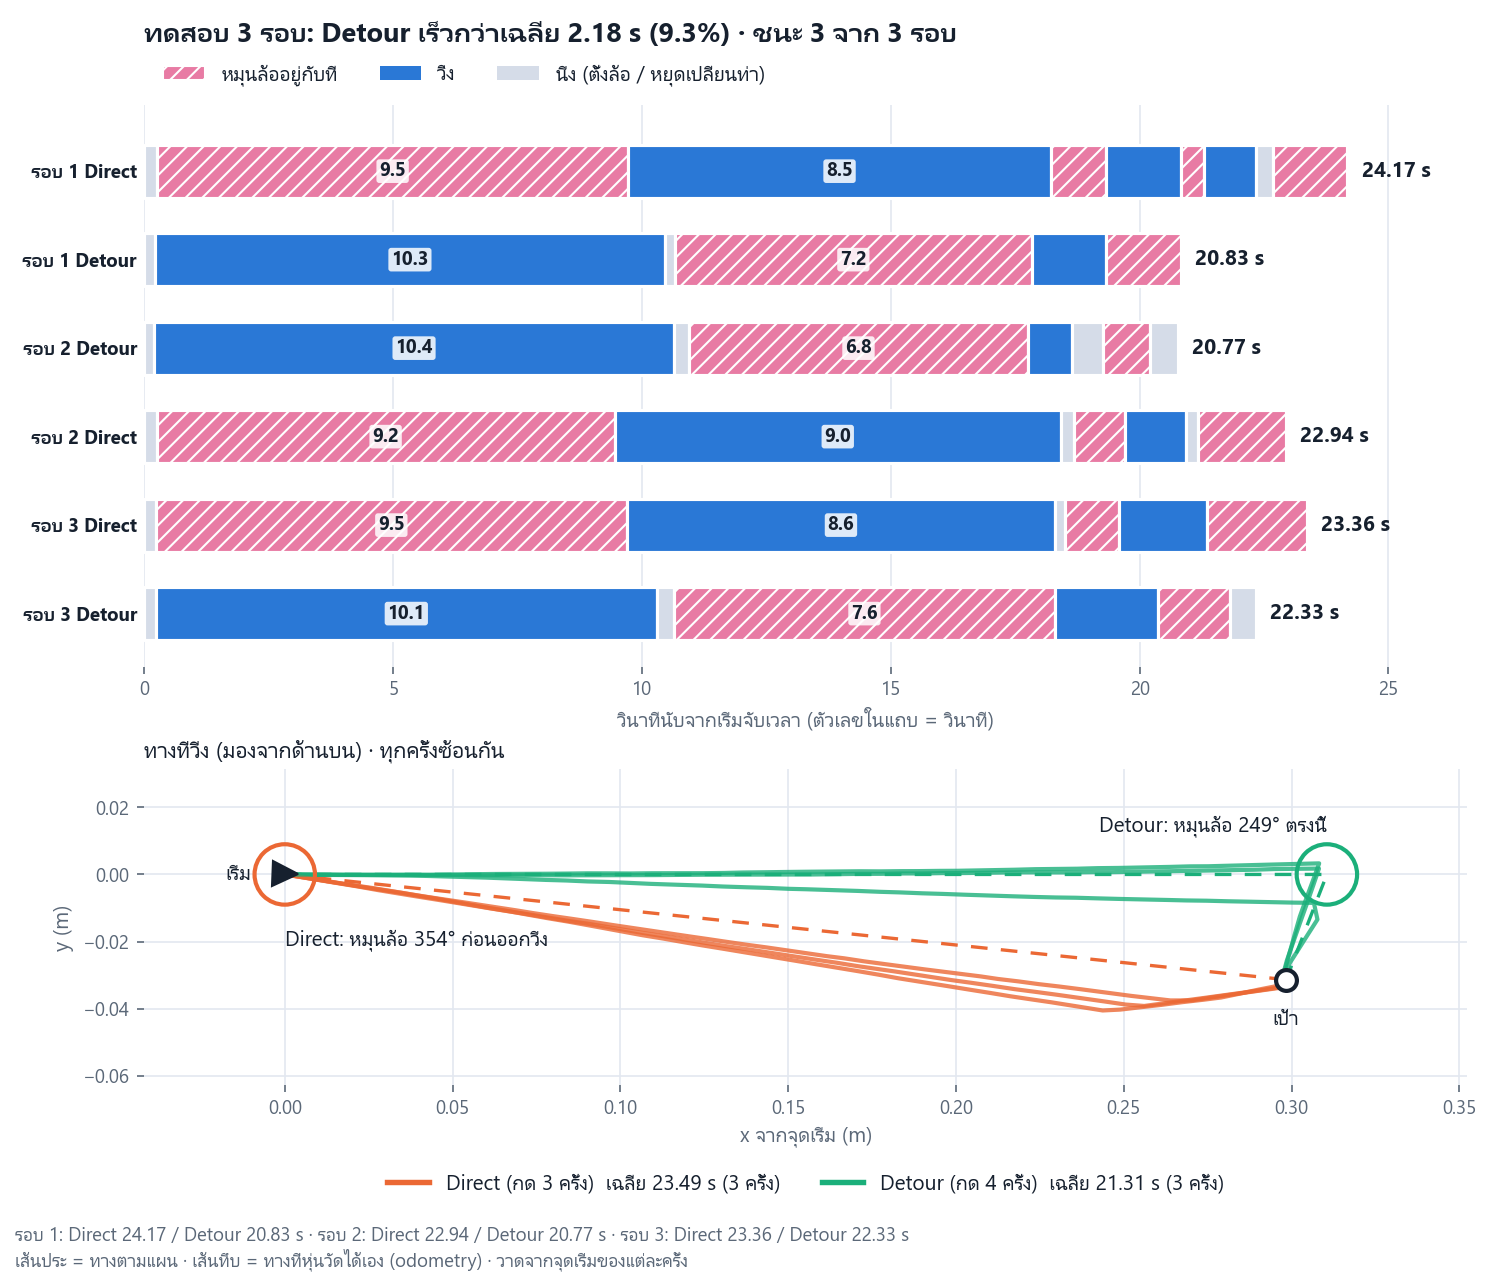
\includegraphics[width=0.74\linewidth]{robot_3rounds.png}\\[-1mm]
{\small Figure 1. The 3 rounds, from the robot's own record (top: time line, bottom: measured paths).}
\end{center}

\section*{6. Conclusion}
One closed-form rule decides between ``steer straight'' and ``drive on, steer less, come back''.
It costs $O(1)$ per decision, is never slower in simulation, and was 9.3\,\% faster on the real robot.
No earlier work found gives this closed-form detour for a robot that must stop to steer one way only
(``not found'' is not proof that nobody did it).

\clearpage
\section*{Code, Git and video}
All code (Python planner, simulators, robot firmware) and the full report:
\begin{center}\large\url{https://github.com/Mannaja78520/mor_luam}\end{center}
\begin{itemize}\setlength\itemsep{0pt}
\item Planner and simulators: \texttt{algorithm\_sim/} (runs without Docker: \texttt{pip install matplotlib}).
\item Robot version: \texttt{firmware/src/algorithm/DetourSteer.cpp}.
\item Full report: \texttt{algorithm\_sim/docs/660610840\_DetourSteer.pdf} (Thai), \texttt{report.pdf} (English).
\item Install guide: \texttt{algorithm\_sim/README.md}, \texttt{docs/INSTALL\_TH.md} (Docker is the recommended install).
\end{itemize}

\textbf{Video of the robot working:}
\begin{center}\url{https://drive.google.com/drive/folders/11qOM6UoeH2c4nEuM0a0JO6eXTnr0eDud}\end{center}
{\small The clip shows the robot working in synchronize mode. There is no clip of the
Detour Steer vs old method (Direct) comparison; that comparison comes from the robot's own record
(Figure 1 and the results table).}
\end{document}
